% !TEX root = SegwayDoku.tex
\renewcommand{\autoren}{Valentyn Chepil}
\newpage
\section{Die Hinderniserkennung}
\subsection{Ultraschallsensor}
% \ref{bild_3} zuweisung auf Bild in Text.

\begin{figure}[h]  % [h] bedeutet, dass das Bild genau an dieser Stelle im Text erscheint
	% mit width=... wird die Größe des Bildes in Prozent der Seitenbreite eingestellt
	\centering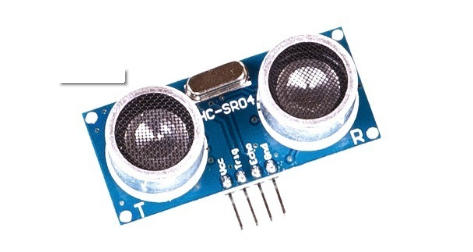
\includegraphics[width=0.5\textwidth]{images/Bilder/Bild 1.1.jpg}
	% caption ist die Bildunterschrift, taucht auch im Abbildungsverzeichnis auf
	\caption{Ultraschallsensor \newline(Quelle: ebay.de)}
	\label{bild_1.1} % über das label kann man aus dem Text auf das Bild verweisen
\end{figure}

Parameter:
\begin{itemize} 
	\item Modul: Hc-SR04 
	\item Preis:  1.50 Doller
	\item Quelle: funduinoshop.com
\end{itemize}

Die Erkennung vom Hindernis erfolgt über ausgehenden Schallwellen, die sich in kegelförmig Form  ausbreiten. Bei Erreichung des Ziels werden die reflektierende Schallwellen aufgenommen und das Zeig des Reflektion wird ausgemessen. Dadurch erkennt man das Hindernis und den Abstand zu dem. Die Ausbreitung und die reflektierende Schallwellen hängt von verschiedenen Faktoren ab. Sie werden vom Luftdruck, der Umgebungstemperatur, der Luftfeuchtigkeit sowie
vom Sende-/Empfangswinkel und der Oberfläche des im Schallkegel befindlichen Objekts
beeinflusst.

  Vorteile:

Ein größter Vorteil des Ultraschallsensors ist günstiger Preis. Dies ermöglicht die Verwendung von vielen Sensoren bei der Modellbau, was zur präzisen Erfassung der Entfernung zu Hindernissen und Objekten in der Umgebung führt.

\begin{figure}[h]  % [h] bedeutet, dass das Bild genau an dieser Stelle im Text erscheint
	\centering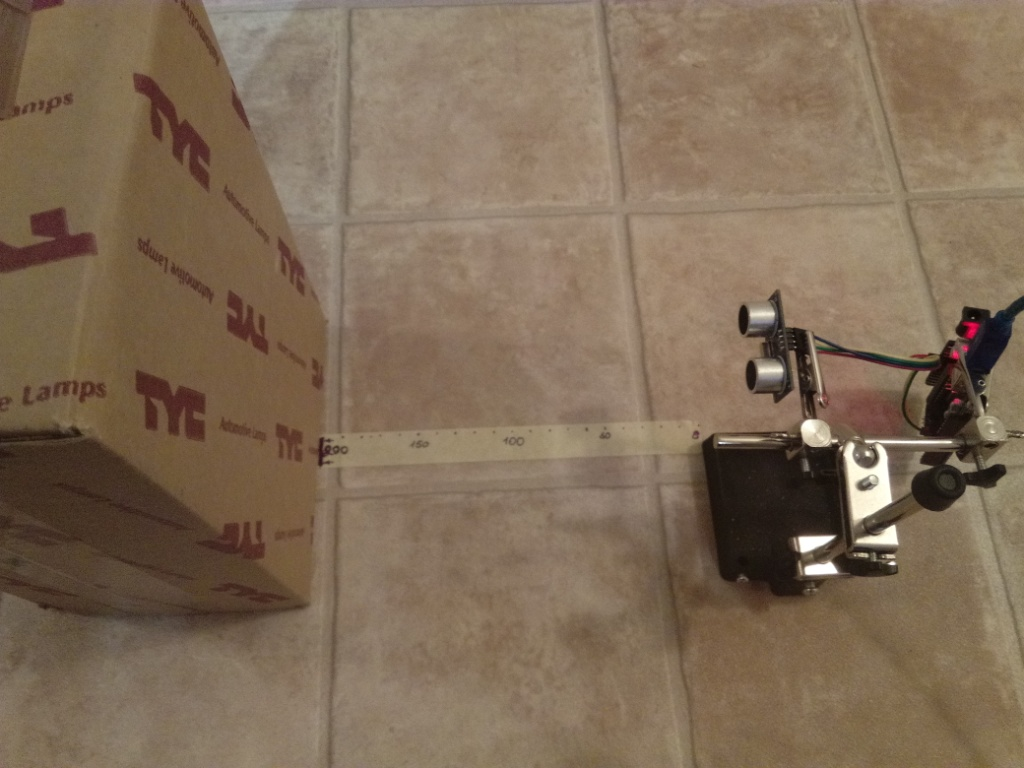
\includegraphics[ width = 0.6\textwidth]{images/Bilder/Bild 1.jpg}
	\caption{Entfernungsmessung \newline (Quelle: eigene Darstellung, US-Sensor Messvorgang)}
	\label{bild_1} % über das label kann man aus dem Text auf das Bild verweisen
\end{figure}



  Nachteile:


Ein Hindernis oder Objekt kann nicht genau geortet werden, sondern man kann nur feststellen, dass es sich in der gemessenen Entfernung innerhalb des Schallkegels befindet. 


\begin{figure}[h]  % [h] bedeutet, dass das Bild genau an dieser Stelle im Text erscheint
	\centering\includegraphics[ width = 0.6 \textwidth]{images/Bilder_USS/Bild_2.png}
	\caption{Positionierung in Messbereich \newline (Quelle: eigene Darstellung)}
	\label{bild_2} % über das label kann man aus dem Text auf das Bild verweisen
\end{figure}

Bei mehrere Objekten vor Schallwelle wird der Abstand zum nächstliegenden Hindernis gemessen und die weit liegender Objekte werde einfach nicht erkannt.


\begin{figure}[h]  % [h] bedeutet, dass das Bild genau an dieser Stelle im Text erscheint
	\centering\includegraphics[width=0.6\textwidth]{images/Bilder_USS/Bild_3.png}
	\caption{Positionierung in Messbereich \newline (Quelle: eigene Darstellung)}
	\label{bild_3} % über das label kann man aus dem Text auf das Bild verweisen
\end{figure}

Als Nachteil kann man nennen die geringe Reichweite (ca. 3m) des Ultraschalls und  der geringen Ausbreitungsgeschwindigkeit des Schalls.

Große Probleme bekommt man auch aus den Reflektionseigenschaften der Schallwellen. Besonders bei weichen Materialien und spitzen-förmigen Oberflächen,
Oberflächenerkennung erfasst das Sensor auch schleicht. Das kann man in der Abbildung \ref{bild_4} und \ref{bild_5} sehen.

\begin{figure}[h]  % [h] bedeutet, dass das Bild genau an dieser Stelle im Text erscheint
	\centering\includegraphics[width=0.6\textwidth]{images/Bilder_USS/Bild_4.jpg}
	\caption{Weiche Material\newline(Quelle: eigene Darstellung,Frauen-Halsschal)}
	\label{bild_4}
\end{figure}

\begin{figure}[h]  % [h] bedeutet, dass das Bild genau an dieser Stelle im Text erscheint
	\centering\includegraphics[width=0.6\textwidth]{images/Bilder_USS/Bild_5.jpg}
	\caption{Spitzen-förmige Oberflächen und weicher Material\newline(Quelle: eigene Darstellung, Teppich)}
	\label{bild_5}
\end{figure}

\begin{figure}[h]  % [h] bedeutet, dass das Bild genau an dieser Stelle im Text erscheint
	\centering\includegraphics[width=0.6\textwidth]{images/Bilder_USS/Bild_6.png}
	\caption{Spitzen-förmige Oberflächen\newline(Quelle: eigene Darstellung, z.B: Kanten)}
	\label{bild_6}
\end{figure}

Wird das Winkel des Schallkegels größer seinem Öffnungswinkel auf eine ebene Wand, so erreicht die Reflektion den aussendenden Sensor nicht. Kann man am Abbildung \ref{bild_7} sehen.

\begin{figure}[h]  % [h] bedeutet, dass das Bild genau an dieser Stelle im Text erscheint
	\centering\includegraphics[width=0.8\textwidth]{images/Bilder_USS/Bild_7.png}
	\caption{Öffnungswinkel (Quelle: eigene Darstellung)}
	\label{bild_7} % über das label kann man aus dem Text auf das Bild verweisen
\end{figure}


 
 
\newpage
 
 
\subsection{Laser Sensor Variante 1}

\begin{figure}[h]  % [h] bedeutet, dass das Bild genau an dieser Stelle im Text erscheint
	\centering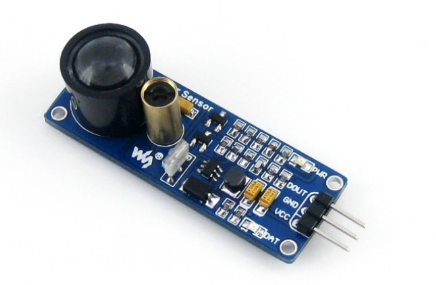
\includegraphics[width=0.6\textwidth]{images/Bilder_USS/laser-sensor.png}
	\caption{Laser-Sensor (Quelle: waveshare.com)}
	\label{laser-sensor} % über das label kann man aus dem Text auf das Bild verweisen
\end{figure}

\begin{itemize}
\item Modul: 
\item Chip-Name: PT1301
\item Preis: 10.79 Doller
\item Quelle: https://www.waveshare.com/Laser-Sensor.htm
\end{itemize}


\begin{figure}[h]  % [h] bedeutet, dass das Bild genau an dieser Stelle im Text erscheint
	\centering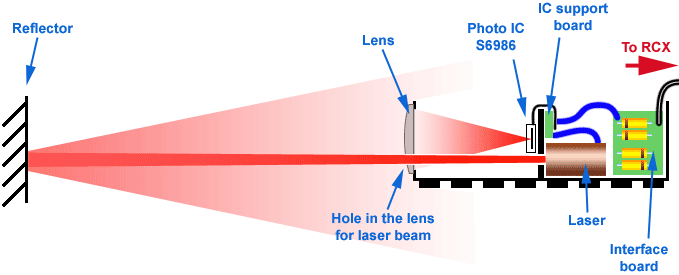
\includegraphics[width=0.9\textwidth]{images/Bilder_USS/laser-sensor1.png}
	\caption{ \ Aufbau der Sensors (Quelle:philohome.com)}
	\label{laser-sensor1} % über das label kann man aus dem Text auf das Bild verweisen
\end{figure}

Text

\newpage
\subsection{Laser Sensor Variante 2}

\begin{figure}[h]  % [h] bedeutet, dass das Bild genau an dieser Stelle im Text erscheint
	\centering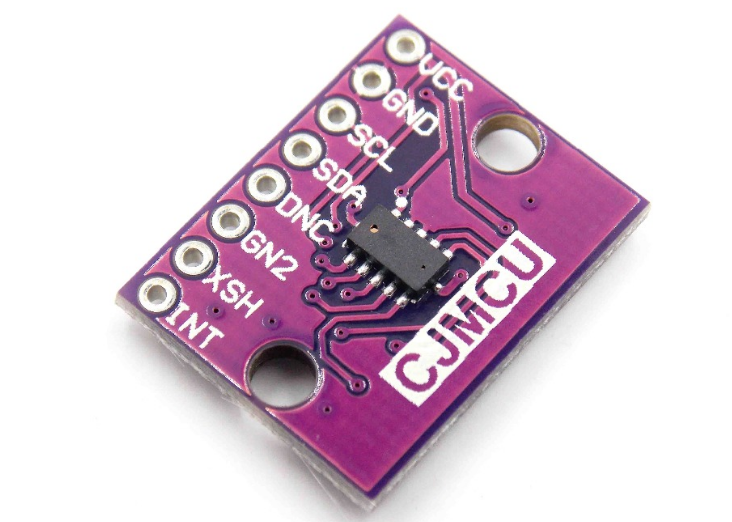
\includegraphics[width=0.6\textwidth]{images/Bilder_USS/laser-sensor_v2.png}
	\caption{ \ Laser-Sensor-VL53L0X (Quelle: ebay.de)}
	\label{laser-sensor_v2} % über das label kann man aus dem Text auf das Bild verweisen
\end{figure}

Parameter:
\begin{itemize}

\item Modul: CJMCU-530
\item Chip-Name: VL53L0X
\item Preis: 4,84 Doller
\end{itemize}



text

\newpage
\subsection{Infrarot Sensor}

\begin{figure}[h]  % [h] bedeutet, dass das Bild genau an dieser Stelle im Text erscheint
	\centering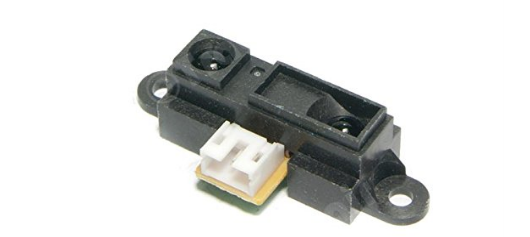
\includegraphics[width=0.8\textwidth]{images/Bilder_USS/infrarot.png}
	\caption{ \ Infrarot-Sensor  (Quelle: amazon.de)}
	\label{infrarot} % über das label kann man aus dem Text auf das Bild verweisen
\end{figure}

\begin{itemize}
\item Modul: 
\item Preis: 1,53 Doller
\item Kommunikation: Analog Output Voltage (typischerweise 0,4 bis 2,3 V Range)
\item Betriebstemperatur:-10 bis + 60 °C
\item Minimale Messdistanz = 10 cm
\item Maximale Messdistanz = 80 cm
\item Reaktionszeit = 38 ± 10 ms

\end{itemize}



Datenblatt – > http://makertreeebayimages.azurewebsites.net/ebayimages/ebaycontent/gp2y0 a21yk-data-sheet.pdf
 
 Dieses Sensor sendet ein Strahl des Infrarot-Licht auf ein Objekt und wartet  reflektierte Licht zurück kommt.